\documentclass[a4paper, 12pt, titlepage]{article}

\usepackage[polish]{babel}	% Enable polish text
\usepackage[utf8]{inputenc}
\usepackage[T1]{fontenc}
\usepackage{times}
\usepackage{anysize}
\usepackage{amsmath}
\usepackage{soul} 			% Strike throught text (\st{}) 

\usepackage{hyperref} % Clickable table of contents
\hypersetup{colorlinks=true,
			allcolors=black,
			urlcolor=cyan}
\usepackage{enumitem} % noitemsep option in lists
\setlist{leftmargin=1.5cm}
\setlist[description]{labelindent=1.1cm, leftmargin=2cm}

\usepackage{datetime} % Enable currenttime  command
% advance the hour register by nr of hours
% negative values if you want to subtract
\advance\currenthour by 1

%\usepackage[none]{hyphenat} % Prevent hyphenation for words
\usepackage{ifthen}			% Enable ifthenelse function
\usepackage{graphicx}		% Enable pictures
\usepackage{alltt}			% Enable non-foramted text input

\marginsize{2cm}{2cm}{2cm}{2cm}


\title{Przetwarzanie obrazów cyfrowych\\
	Opracowanie pytań do egzaminu}
%\author{Vadym Perepeliak}


%%%%%%%%%%%%%%%%%
\begin{document}
\maketitle
\tableofcontents
\pagebreak
    
    
%%%%%%%%%%%%%%%%%%%%%%%%%%%%%%%%%%%%%%%%%%%%%%%%%%%%%%%%%%%%%%%%%%%%%%%%%%%%%%%%%%%%%%%
\pagebreak\section{Budowa oka i proces widzenia}

\subsection{Metody ekstrakcji (rozpoznania) tęczówki oka}
TODO. Aby zidentyfikować użytkownika, wykonuje się obraz tęczówki (w podczerwieni bądź świetle widzialnym), a następnie oprogramowanie usuwa z obrazu zakłócenia (np.: źrenicę, rzęsy). 

\subsection{Wymień elementy oka skupiające obraz na siatkówce}
Światło przechodzi przez rogówkę, źrenice regulowaną tęczówką – kolorową częścią oka, soczewkę, która załamuje promienie świetlne, ciało szkliste. Potem promienie padają na wewnętrzną warstwę oka – siatkówkę gdzie powstaje odwrócony obraz.

\subsection{Za co odpowiedzialne są pręciki w oku}
Pręciki mają wysoką czułość, przeznaczone do widzenia nocnego, odpowiedzialne za wykrywanie kształtu i ruchu. Brak czułości na barwę.

\subsection{Wymienić elementy siatkówki i punkty charakterystyczne na siatkówce}
Siatkówka składa się z fotoreceptorów – czopków (odpowiedzialne za kolor) i pręcików (odpowiedzialne za widzenie nocne), plamki żółtej – największe skupisko czopków oraz plamki ślepej – tam nie ma fotoreceptorów, od niej wychodzi nerw wzrokowy.

%%%%%%%%%%%%%%%%%%%%%%%%%%%%%%%%%%%%%%%%%%%%%%%%%%%%%%%%%%%%%%%%%%%%%%%%%%%%%%%%%%%%%%%
\pagebreak\section{Sztuczne systemy wizyjne}

\subsection{Podaj min. 3 cechy naturalnego przetwarzania obrazu przewyższające sztuczne przetwarzanie obrazu}
\begin{itemize}[noitemsep]
	\item Szybka analiza złożonych obrazów
	\item Większa skuteczność rozpoznawania obrazów dwuznacznych
	\item Łatwe i efektywne uczenie się nowych schematów
	\item Szybsze rozpoznawanie obrazów w czasie rzeczywistym
\end{itemize}

\subsection{Podaj dwie nowoczesne metody sztucznego przechwytywania obrazu i krótko je opisz. \\ 2 metody akwizycji obrazu w kamerach}
\begin{description}
	\item[Lampa analizująca] - stosowane zjawisko fotoelektryczne, w rezultacie powstaje obraz monochromatyczny. Zarejestrowanie kolorów wymaga współdziałania trzech lamp, do których jest doprowadzone światło rozbite na barwy podstawowe RGB.
	\item[CCD] (Układ ze sprężeniem ładunkowym) - półprzewodnikowa matryca złożona z milionów światłoczułych elementów (fotodiod). W poszczególnych diodach gromadzi się ładunek elektryczny, proporcjonalny do liczby padających fotonów.
\end{description}

\subsection{2 sposoby według których czujniki światła reagujące tylko na jego natężenie mogą rozróżniać kolory}
\begin{itemize}
	\item Specjalne filtry barwne, selektywnie dostarczające do poszczególnych pikseli jedną składową barwną $\rightarrow$ powstały obraz ma niższą jakość i rozdzielczość
	\item W układzie optycznym kamery światło rozszczepiane na składowe RGB, kierując go poprzez filtry widmowe na trzy elementy CCD $\rightarrow$ pewna rozdzielczość obrazu.
\end{itemize}

\subsection{Przyporządkuj parametry do standardów telewizyjnych. \\ NTSC i PAL wybrać odpowiednią ilość Hz i linii na pół-obrazie. \\ Liczba linii PAL, półobrazów i obrazów w czasie 1 sek}
\begin{description}
	\item[PAL] - 625 linii, 25 obrazów/s, częstotliwość odświeżania 50 Hz
	\item[NTSC] - 575 linii, 30 obrazów/s, częstotliwość odświeżania 60 Hz
\end{description}
	
\subsection{Czujniki CCD wykazują największą czułość dla fal...}
1050 nm - podczerwień
%%%%%%%%%%%%%%%%%%%%%%%%%%%%%%%%%%%%%%%%%%%%%%%%%%%%%%%%%%%%%%%%%%%%%%%%%%%%%%%%%%%%%%%
\pagebreak\section{Modele barw}

\subsection{Połącz przestrzenie barw z zastosowaniem}
\begin{description}[noitemsep, labelwidth=1.7cm]
	\item[CMY(K)] -	poligrafia (druk)
	\item[HSV] - w programach graficznych
	\item[RGB] - naturalne postrzeganie barw, ekran komputera i telewizora
	\item[YCrCb] - przesyłanie i przechowywanie wideo
	\item[YUV] - przesyłanie danych, analogowa TV (zgodność z czarno-białą - samo Y). Model YUV był wykorzystywany w czasie przechodzenia od telewizorów czarno-białych na kolorowe. Kamerka w smarfonie zapisuje w YUV
\end{description}

\subsection{Co to równomierna percepcyjnie przestrzeń barw (np CIE Lab) ?}
To taka przestrzeń barw, w której obszary różnicy percepcyjnej barw mają postać kul o jednakowym promieniu w obrębie całej przestrzeni barw. \par
Przestrzeń barw CIELab i CIELUV pretendują do miana równomiernych przestrzeni barw jednak faktycznie są jej przybliżeniem. (\href{https://pl.wikipedia.org/wiki/R%C3%B3wnomierna_przestrze%C5%84_barw}{link do Wikipedii})
	
\subsection{Kodowanie CMYK a CMY. \\ Co to K w modelu CMY/CMYK}
CMY(Cyan, Magenta(purpurowy), Yellow) - subtraktywny model barwny.
Z powodu niedoskonałości tuszów stosowanych w urządzeniach do druku, dodając takie same ilości kolorów CMY, nie uzyskamy głębokiej czerni, tylko w większości przypadków kolor ciemno brązowy. Aby zlikwidować ten problem, do zestawu kolorów CMY sdecydowano dodać barwę czarną K = min(C, M, Y).\par
K to minimum z C, M i Y albo osobny kolor czerni.

\subsection{Czerwony w YCrCb zawarty jest w…}
Odp: Cr. Y\textquoteright~is the luma component and Cb and Cr are the blue-difference and red-difference chroma components.

\subsection{Jakie wartości w CMY dadzą kolor niebieski}
C(255) M(255) Y(0) \\
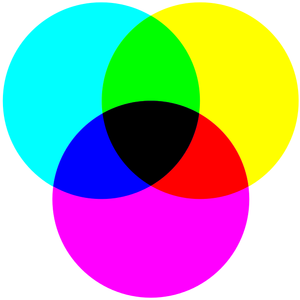
\includegraphics[scale=0.8]{CMY_ideal.png}

\subsection{Kodowanie CMY(jak otrzymać z RGB)}
$\begin{bmatrix} C \\ M \\ Y \\ \end{bmatrix} 
= \begin{bmatrix} 1 \\ 1 \\ 1 \\ \end{bmatrix}
- \begin{bmatrix} R \\ G \\ B \\ \end{bmatrix} $

\subsection{Czym jest Y w YUV.}
Y – luminacja (dla obrazu monochromatycznego), U – składowa niebieska, V – składowa czerwona.
\subsection{Opisać CIE Lab}
\textbf{CIELab} – przestrzeń barw, która została znormalizowana w 1976 przez CIE (Międzynarodową Komisję Oświetleniową). Barwę opisują matematycznie trzy składowe: L - jasność (luminancja), a – barwa od zielonej do magenty, b – barwa od niebieskiej do żółtej.
%%%%%%%%%%%%%%%%%%%%%%%%%%%%%%%%%%%%%%%%%%%%%%%%%%%%%%%%%%%%%%%%%%%%%%%%%%%%%%%%%%%%%%%
\pagebreak\section{Rozdzielczość i skalowanie}

\subsection{Czym się różni Nearest Neighbour od interpolacji}
W metodzie Nearest Neighbour brany jest pod uwagę tylko jeden najbliższy piksel. W metodzie interpolacji brane pod uwagę są piksele otoczenia np. 8 pikseli dla okna 3x3.

\subsection{Skalujemy obraz sztuczny przedstawiający szachownicę do wyższej rozdzielczości. Stosujemy metodę najbliższego sąsiada oraz metodę interpolacji. Która metoda będzie lepsza i dlaczego?}
Lepsza będzie metoda najbliższego sąsiada, która dla obrazów z niewielką ilością stopni szarości (sztucznych) nie powoduje zniekształceń wynikających z uwzględniania otoczenia piksela jak w metodzie interpolacji.

\subsection{Mamy czarno-białą kratownice i ją powiększamy. Stosujemy metodę najbliższego sąsiada oraz metodę interpolacji. Która metoda będzie lepsza i dlaczego?}
Wyniki będą podobne dla czarno-białego obrazu. Jednak metoda interpolacji może dać lepszy obraz ze względu na linii inne od poziomych i pionowych, ponieważ jest brana pod uwagę otoczenie piksela.

\subsection{Co to jest 720p}
Termin ten wskazuje, że obraz ma 720 linii poziomych. W formacie 16:9 jest to
obraz o wymiarach 1280x720. Literka ‘p’ wskazuje, że obraz jest bez przeplotu.

\subsection{Co to jest 1080i}
Określa rozdzielczość obrazu równą 1920x1080. Literka ‘i’ wskazuje, że obraz jest
z przeplotem (naprzemienne wyświetlanie parzystych i nieparzystych linii obrazu). \par
Literka p - \textbf{progressive scan} czyli wyświetlane we wszystkich klatkach pełne
obrazy. Literka i - \textbf{interlaced} czyli z przeplotem wyświetlane są pół-obrazy.
Lepsze jest z \textbf{p}.

%%%%%%%%%%%%%%%%%%%%%%%%%%%%%%%%%%%%%%%%%%%%%%%%%%%%%%%%%%%%%%%%%%%%%%%%%%%%%%%%%%%%%%%
\pagebreak\section{Przekształcenia obrazu}

\subsection{2 metody normalizacji}
\begin{description}[noitemsep]
	\item[Skalowanie z obcięciem] - dodajemy/odejmujemy pewną wartość i usuwamy wartości poza zakresem.
	\item[Skalowanie bez obcięcia] dodajemy/odejmujemy najmniejszą wartość a następnie dzielimy wszystko tak by największa wartość była równa maksymalnej możliwej wartości
\end{description}

\subsection{Opisać operację LUT}
Operacja korzysta z gotowych tabel przekodowania look-up tables, w których dla każdej wartości piksela oryginalnego obrazu mamy gotową wartość piksela nowego obrazu.

\subsection{Wybrać operacje bezkontekstowe}
Operacje bezkontekstowe: LUT, negacja, negatyw, wyrównanie histogramu, dodawanie, odejmowanie, mnożenie, \st{filtr morfologiczny}, \st{mediana}

\subsection{Jak zrobić przekształcenie punktowe nie mając danego przepisu analitycznego}
???

\subsection{Coś o współczynnikach normalizacji w maskach - dla podanych masek 3x3 podać ich współczynniki normalizacyjne}
Współczynnik normalizacji W to jest suma wag w masce.
$$ W = \sum w(i,j) $$
Dla maski: 
\begin{tabular}{|c|c|c|}
	\hline
	1 & 4 & 1 \\ \hline
	4 & 3 & 4 \\ \hline
	1 & 4 & 1 \\ \hline
\end{tabular} W = 23 
%%%%%%%%%%%%%%%%%%%%%%%%%%%%%%%%%%%%%%%%%%%%%%%%%%%%%%%%%%%%%%%%%%%%%%%%%%%%%%%%%%%%%%%
\pagebreak\subsection{Histogram obrazu}

\subsection{Opisać krótko algorytm wyrównywania histogramu (HE)}
Etapy równoważenia histogramu:
\begin{enumerate}
	\item Obliczenie histogramu skumulowanego (suma pikseli dla poszczególnych poziomów szarości + suma poprzednich poziomów).
	\item Normalizacja histogramu skumulowanego (dzielenie przez sumę pikseli).
	\item Pomnożenie wartości otrzymanych w pkt.2 przez maksymalną wartość poziomu szarości i zaokrąglenie do liczb naturalnych.
	\item Utworzenie obrazu wynikowego poprzez przypisanie pikselom na poszczególnych poziomach szarości nowych wartości wyliczonych w poprzednich krokach.
\end{enumerate}


\subsection{Histogram BBHE i DISHE, czym się charakteryzują i po co są \\ Dlaczego metody BBHE i DISHE są lepsze od klasycznego wyrównywania histogramu HE?}
Klasyczne wyrównywanie histogramu HE ma jedną zasadniczą wadę: po wykonaniu operacji
jasność obrazu ulega zmianie. Metody, które eliminują to niekorzystne zjawisko polegają na dekompozycji obrazu wejściowego na dwa podobrazy (wg. pewnego kryterium) i wykonania operacji HE dla tych podobrazów. 
\begin{description}
	\item[BBHE] (Bi-Histogram Equalization) - kryterium podziału to średnia jasność w obrazie.
	\item[DSIHE] (Dualistic Sub-Image Histogram Equalization) - obraz dzielony jest na dwa podobrazy o takiej samej ilości pikseli (jaśniejszych i ciemniejszych) 
\end{description}

%%%%%%%%%%%%%%%%%%%%%%%%%%%%%%%%%%%%%%%%%%%%%%%%%%%%%%%%%%%%%%%%%%%%%%%%%%%%%%%%%%%%%%%
\pagebreak\section{Binaryzacja}
\subsection{Jedna metoda znajdowania progu binaryzacji + opis}
Próg binaryzacji możemy znaleźć analizując histogram obrazu. Na ogół będziemy mieć do czynienia z dwiema “górkami” pikseli - jedna to piksele obiektu, drugie tła (jasne obiekty na ciemnym tle lub na odwrót). Próg dobieramy biorąc wartość pomiędzy nimi, w dolinie. Pozwoli to na oddzielenie obiektów od tła.

\subsection{Znajdowanie progu binaryzacji metodą histerezy + opis \\ Wyjaśnij na czym polega binaryzacja z histerezą}
Progowanie z histerezą stosuje się w przypadkach, gdy klasy pikseli w histogramie nie są wyraźnie rozseparowane, np. gdy granice obiektu w obrazie są rozmazane, niewyraźne. W takim przypadku definiuje się dwa progi: lewy oraz prawy. Wartości leżące poniżej progu lewego definiują część główną obiektu, wartości leżące powyżej progu prawego wyznaczają tło. Wartości między lewym a prawym progiem są klasyfikowane jako reprezentujące obiekt pod warunkiem, że piksel przyjmujący taką wartość sąsiaduje w obrazie z pikselem należącym do głównego obiektu.\\
% TODO: przerobić na latex
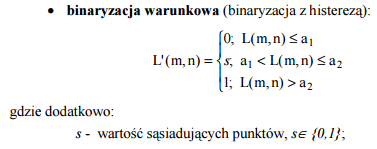
\includegraphics[scale=0.8]{Bin_histereza_wzor.png} 
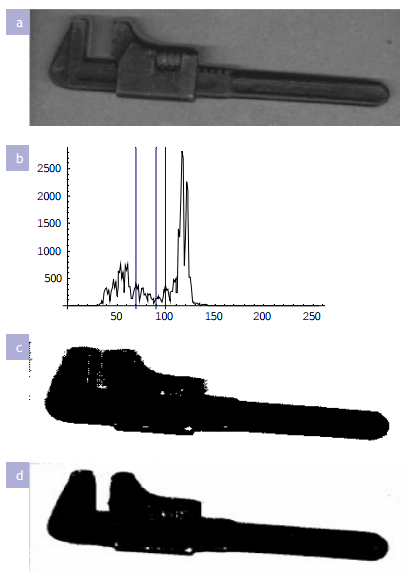
\includegraphics[scale=0.8]{Bin_histereza.png}

\subsection{Ryż na obrazku się źle zbinaryzował (jakieś plany czarne itp) i trzeba napisać jak się tego pozbyć (wykorzystano metodę Savouli)}
???

\subsection{Podaj przykład metody automatycznego wyznaczania progu binaryzacji. Na podstawie czego jest wyznaczany?}
Metoda Otsu - automatycznie testuje się różne progi i szuka takiego progu, dla którego wariancja międzygrupowa będzie najwyższa a wariancja wewnątrzgrupowa będzie najniższa. Wynik uzyskujemy poprzez analizę średnich ważonych w komponentach.

\subsection{Kiedy używa się binaryzacji lokalnej}
W przypadku niejednorodnie oświetlonego obrazu.\\
Krótki opis binaryzacji lokalnej:
\begin{enumerate}[noitemsep]
	\item Podziel obraz na rozłączne kratki np. 8x8 pikseli
	\item W każdej kratce wyznacz próg binaryzacji (np. za pomocą Otsu)
	\item Dla każdego piksela użyj lokalnego progu, który jest przybliżony za pomocą 4 najbliższych progów.
\end{enumerate}
%%%%%%%%%%%%%%%%%%%%%%%%%%%%%%%%%%%%%%%%%%%%%%%%%%%%%%%%%%%%%%%%%%%%%%%%%%%%%%%%%%%%%%%
\pagebreak\section{Filtracja kontekstowa}

\subsection{Filtracja kontekstowa - opisać}
Oznacza że dla wyznaczenia wartości jednego punktu obrazu wynikowego trzeba dokonać obliczenia na wielu punktach obrazu oryginalnego, z reguły na punktach sąsiednich.

\subsection{Dlaczego w filtracji górnoprzepustowej nie stosuje się normalizacji tak jak w filtracji dolnoprzepustowej?}
??? Chyba powinno być na odwrót. Normalizacja jest stosowana w filtrach górnoprzepustowych. \\
Ponieważ w maskach filtrów górnoprzepustowych są ujemne współczynniki wag, w obrazach wynikowych wartości piksele mogą wykroczyć poza zakres 0-255. W filtrach dolnoprzepustowych takie zjawisko nie występuje bo niema ujemnych wag.

\subsection{Jak działa filtr medianowy? \\ Podany obraz, jak będzie wyglądał środkowy piksel po filtracji medianowej?}
Bierze pod uwagę środkową wartość (medianę) uporządkowanych pikseli z otoczenia rozważanego piksela. Ekstremalne wartości nie wpływają na jego działanie. Bardzo skutecznie zwalcza szumy, nie powodując ich rozmazywania na większym obszarze. Nie wprowadza do obrazu nowych wartości, więc obraz po filtracji nie wymaga skalowania. Nie powoduje pogorszenia ostrości krawędzi, ale ma tendencję do zjadania narożników.

\subsection{Czy filtr medianowy z oknem 5x5 całkowicie odfiltruje zakłócenia o (ciemne zakłócenie na jasnym tle) dla zakłócenia o rozmiarze: 2x4, 3x5, 6x5, 2x14?}
Będą odfiltrowane zakłócenia tylko o rozmiarach 2x4 i 3x5, bo zakłócenia o rozmiarach 6x5 i 2x14 nie mieszczą się w oknie filtra.

\subsection{Za pomocą, których masek można otrzymać filtr kombinowany \\ Jakie gradienty można zastosować w filtrach kombinowanych \\ Jakie filtry mogą być kombinowane}
Za pomocą dwóch prostopadłych (w różnych kierunkach) masek Sobela (Prewitta, Robertsa) i kombinacji Euklidesowej lub modułowej. Nazywane: "gradient Sobela", "gradient Prewitta", "gradient Robertsa" "gradient Kirscha" (nie był omawiany ale istnieje). \\
Kombinacja Euklidesowa:
$$ L^{\prime}(m,n) = \sqrt{(L_{1}(m,n))^2+(L_{2}(m,n))^2} $$
Uproszczona formuła modułowa:
$$ L^{\prime}(m,n) = |(L_{1}(m,n)|+|L_{2}(m,n)| $$

\subsection{Filtracja adaptacyjna - opisać \\ Co wykrywa filtr adaptacyjny w pierwszym etapie działania? \\ Jaki jest drugi etap jego działania? \\ W jakim celu może być zastosowany filtr adaptacyjny?}
Filtry adaptacyjne zmieniają charakterystykę działania w zależności od cech analizowanego obrazu. Filtry te działają dwuetapowo:
\begin{enumerate}[noitemsep]
	\item W pierwszym etapie wyznaczamy czy należy dany punkt do krawędzi. Jako kryterium można przyjąć różnice stopni szarości w jego otoczeniu.
	\item Dokonuje się filtracji filtrem uśredniającym ale tylko dla punktów które nie należą do krawędzi. Punkty krawędzi pozostają bez zmian.
\end{enumerate}
Zastosowania:
\begin{itemize}[noitemsep]
	\item Wyrównanie intensywności poszczególnych płaszczyzn nie rozmazując krawędzie.
	\item Wzmocnienie krawędzi bez niepotrzebnych szczegółów w jednolitych obszarach.
\end{itemize}

\subsection{Wybrać filtr liniowy z podanych}
Filtry liniowe: Uśredniający, Robertsa, Prewitta, Sobela, Laplasjany

\subsection{Zaproponuj maskę do wykrycia krawędzi poziomych}
Maska Sobela:
\begin{tabular}{|c|c|c|}
	\hline
	1 & 2 & 1 \\ \hline
	0 & 0 & 0 \\ \hline
	-1 & -2 & -1 \\ \hline
\end{tabular}
\subsection{Podaj przykład maski wykrywające krawędzie pionowe}
Maska Sobela:
\begin{tabular}{|c|c|c|}
	\hline
	1 & 0 & -1 \\ \hline
	2 & 0 & -2 \\ \hline
	1 & 0 & -1 \\ \hline
\end{tabular}

\subsection{Maska 3x3 wykrywająca krawędzie pionowe + zaznaczenie na obrazie wynikowym krawędzi wykrytej + zastosowanie filtracji medianowej 3x3}
Maska Sobela wykrywajace krawędzie pionowe:
\begin{tabular}{|c|c|c|}
	\hline
	1 & 0 & -1 \\ \hline
	2 & 0 & -2 \\ \hline
	1 & 0 & -1 \\ \hline
\end{tabular}.
Filtracja medianowa: Bierze pod uwagę środkową wartość (medianę) uporządkowanych pikseli z otoczenia rozważanego piksela.

\subsection{Jaka maska z podanych wyostrzy krawędzie}
Przykładowe maski laplasjany do wykrywania krawędzie:
\begin{tabular}{|c|c|c|}
	\hline
	0 & -1 & 0 \\ \hline
	-1 & 4 & -1 \\ \hline
	0 & -1 & 0 \\ \hline
\end{tabular}
\begin{tabular}{|c|c|c|}
	\hline
	-1 & -1 & -1 \\ \hline
	-1 & 8 & -1 \\ \hline
	-1 & -1 & -1 \\ \hline
\end{tabular}

\subsection{Podana zlogarytmowana wizualizacja amplitudy jakiegoś filtra. Jaki to filtr? dolnoprzepustowy górnoprzepustowy, zaporowy?}
???

\subsection{Obraz Lena z samymi krawędziami, która filtracja wykonana: dolnoprzepustowa, górnoprzepustowa, przemnożenie przez stałą}
Racej górnoprzepustowa skoro są same krawędzie.

\subsection{Z czego składa się filtr gabora}
???

\subsection{Wykres 3D filtra, jaki to filtr: dolnoprzepustowy, górno-, środkowozaporowy, środkowoprzepustowy}
???

\subsection{Różnice pomiędzy filtracją bilateralną a non local means}
Filtracja bilateralna polega na tym, że wartość piksela zastępuje się bardzo specjalną średnią z pikseli otoczenia analizowanego piksela. Nie jest to zwykła średnia arytmetyczna, lecz średnia ważona, w której wagami są zarówno odległość piksela otoczenia od badanego piksela, ale także różnica w cechach radiometrycznych np. intensywności. W efekcie tego zachowane są ostre krawędzie. 
Filtracja non-local means robi tak samo ale uśrednianie obejmuje wszystkie piksele w obrazie. 


%%%%%%%%%%%%%%%%%%%%%%%%%%%%%%%%%%%%%%%%%%%%%%%%%%%%%%%%%%%%%%%%%%%%%%%%%%%%%%%%%%%%%%%
%%%%%%%%%%%%%%%%%%%%%%%%%%%%%%%%%%%%%%%%%%%%%%%%%%%%%%%%%%%%%%%%%%%%%%%%%%%%%%%%%%%%%%%

\end{document}